% This file is generated by the MATLAB m-file laprint.m. It can be included
% into LaTeX documents using the packages graphicx, color and psfrag.
% It is accompanied by a postscript file. A sample LaTeX file is:
%    \documentclass{article}\usepackage{graphicx,color,psfrag}
%    \begin{document}% This file is generated by the MATLAB m-file laprint.m. It can be included
% into LaTeX documents using the packages graphicx, color and psfrag.
% It is accompanied by a postscript file. A sample LaTeX file is:
%    \documentclass{article}\usepackage{graphicx,color,psfrag}
%    \begin{document}% This file is generated by the MATLAB m-file laprint.m. It can be included
% into LaTeX documents using the packages graphicx, color and psfrag.
% It is accompanied by a postscript file. A sample LaTeX file is:
%    \documentclass{article}\usepackage{graphicx,color,psfrag}
%    \begin{document}% This file is generated by the MATLAB m-file laprint.m. It can be included
% into LaTeX documents using the packages graphicx, color and psfrag.
% It is accompanied by a postscript file. A sample LaTeX file is:
%    \documentclass{article}\usepackage{graphicx,color,psfrag}
%    \begin{document}\input{noiserobustness}\end{document}
% See http://www.mathworks.de/matlabcentral/fileexchange/loadFile.do?objectId=4638
% for recent versions of laprint.m.
%
% created by:           LaPrint version 3.16 (13.9.2004)
% created on:           01-Jun-2015 14:29:34
% eps bounding box:     10.2857 cm x 6.7688 cm
% comment:              
%
\begin{psfrags}%
\psfragscanon%
%
% text strings:
\psfrag{s01}[][]{\color[rgb]{0,0,0}\setlength{\tabcolsep}{0pt}\begin{tabular}{c}Average residual\end{tabular}}%
\psfrag{s03}[][]{\color[rgb]{0,0,0}\setlength{\tabcolsep}{0pt}\begin{tabular}{c}Noise parameter $\sigma$\end{tabular}}%
\psfrag{s04}[][]{\color[rgb]{0,0,0}\setlength{\tabcolsep}{0pt}\begin{tabular}{c}ShapeFit for $n=50$, $q=0.2$\end{tabular}}%
%
% axes ticklabel color:
\color[rgb]{0.15,0.15,0.15}%
%
% xticklabels:
\psfrag{x01}[t][t]{$10^{-6}$}%
\psfrag{x02}[t][t]{$10^{-5}$}%
\psfrag{x03}[t][t]{$10^{-4}$}%
\psfrag{x04}[t][t]{$10^{-3}$}%
\psfrag{x05}[t][t]{$10^{-2}$}%
\psfrag{x06}[t][t]{$10^{-1}$}%
\psfrag{x07}[t][t]{$10^{0}$}%
%
% yticklabels:
\psfrag{v01}[r][r]{$10^{-6} \hspace{-0.1em}$}%
\psfrag{v02}[r][r]{}%
\psfrag{v03}[r][r]{$10^{-4}$}%
\psfrag{v04}[r][r]{}%
\psfrag{v05}[r][r]{$10^{-2}$}%
\psfrag{v06}[r][r]{}%
\psfrag{v07}[r][r]{$10^{0}\ \hspace{0.1825em} $}%
%
% Figure:
\resizebox{9cm}{!}{\includegraphics{noiserobustness.eps}}%
\end{psfrags}%
%
% End noiserobustness.tex
\end{document}
% See http://www.mathworks.de/matlabcentral/fileexchange/loadFile.do?objectId=4638
% for recent versions of laprint.m.
%
% created by:           LaPrint version 3.16 (13.9.2004)
% created on:           01-Jun-2015 14:29:34
% eps bounding box:     10.2857 cm x 6.7688 cm
% comment:              
%
\begin{psfrags}%
\psfragscanon%
%
% text strings:
\psfrag{s01}[][]{\color[rgb]{0,0,0}\setlength{\tabcolsep}{0pt}\begin{tabular}{c}Average residual\end{tabular}}%
\psfrag{s03}[][]{\color[rgb]{0,0,0}\setlength{\tabcolsep}{0pt}\begin{tabular}{c}Noise parameter $\sigma$\end{tabular}}%
\psfrag{s04}[][]{\color[rgb]{0,0,0}\setlength{\tabcolsep}{0pt}\begin{tabular}{c}ShapeFit for $n=50$, $q=0.2$\end{tabular}}%
%
% axes ticklabel color:
\color[rgb]{0.15,0.15,0.15}%
%
% xticklabels:
\psfrag{x01}[t][t]{$10^{-6}$}%
\psfrag{x02}[t][t]{$10^{-5}$}%
\psfrag{x03}[t][t]{$10^{-4}$}%
\psfrag{x04}[t][t]{$10^{-3}$}%
\psfrag{x05}[t][t]{$10^{-2}$}%
\psfrag{x06}[t][t]{$10^{-1}$}%
\psfrag{x07}[t][t]{$10^{0}$}%
%
% yticklabels:
\psfrag{v01}[r][r]{$10^{-6} \hspace{-0.1em}$}%
\psfrag{v02}[r][r]{}%
\psfrag{v03}[r][r]{$10^{-4}$}%
\psfrag{v04}[r][r]{}%
\psfrag{v05}[r][r]{$10^{-2}$}%
\psfrag{v06}[r][r]{}%
\psfrag{v07}[r][r]{$10^{0}\ \hspace{0.1825em} $}%
%
% Figure:
\resizebox{9cm}{!}{\includegraphics{noiserobustness.eps}}%
\end{psfrags}%
%
% End noiserobustness.tex
\end{document}
% See http://www.mathworks.de/matlabcentral/fileexchange/loadFile.do?objectId=4638
% for recent versions of laprint.m.
%
% created by:           LaPrint version 3.16 (13.9.2004)
% created on:           01-Jun-2015 14:29:34
% eps bounding box:     10.2857 cm x 6.7688 cm
% comment:              
%
\begin{psfrags}%
\psfragscanon%
%
% text strings:
\psfrag{s01}[][]{\color[rgb]{0,0,0}\setlength{\tabcolsep}{0pt}\begin{tabular}{c}Average residual\end{tabular}}%
\psfrag{s03}[][]{\color[rgb]{0,0,0}\setlength{\tabcolsep}{0pt}\begin{tabular}{c}Noise parameter $\sigma$\end{tabular}}%
\psfrag{s04}[][]{\color[rgb]{0,0,0}\setlength{\tabcolsep}{0pt}\begin{tabular}{c}ShapeFit for $n=50$, $q=0.2$\end{tabular}}%
%
% axes ticklabel color:
\color[rgb]{0.15,0.15,0.15}%
%
% xticklabels:
\psfrag{x01}[t][t]{$10^{-6}$}%
\psfrag{x02}[t][t]{$10^{-5}$}%
\psfrag{x03}[t][t]{$10^{-4}$}%
\psfrag{x04}[t][t]{$10^{-3}$}%
\psfrag{x05}[t][t]{$10^{-2}$}%
\psfrag{x06}[t][t]{$10^{-1}$}%
\psfrag{x07}[t][t]{$10^{0}$}%
%
% yticklabels:
\psfrag{v01}[r][r]{$10^{-6} \hspace{-0.1em}$}%
\psfrag{v02}[r][r]{}%
\psfrag{v03}[r][r]{$10^{-4}$}%
\psfrag{v04}[r][r]{}%
\psfrag{v05}[r][r]{$10^{-2}$}%
\psfrag{v06}[r][r]{}%
\psfrag{v07}[r][r]{$10^{0}\ \hspace{0.1825em} $}%
%
% Figure:
\resizebox{9cm}{!}{\includegraphics{noiserobustness.eps}}%
\end{psfrags}%
%
% End noiserobustness.tex
\end{document}
% See http://www.mathworks.de/matlabcentral/fileexchange/loadFile.do?objectId=4638
% for recent versions of laprint.m.
%
% created by:           LaPrint version 3.16 (13.9.2004)
% created on:           01-Jun-2015 14:29:34
% eps bounding box:     10.2857 cm x 6.7688 cm
% comment:              
%
\begin{psfrags}%
\psfragscanon%
%
% text strings:
\psfrag{s01}[][]{\color[rgb]{0,0,0}\setlength{\tabcolsep}{0pt}\begin{tabular}{c}Average residual\end{tabular}}%
\psfrag{s03}[][]{\color[rgb]{0,0,0}\setlength{\tabcolsep}{0pt}\begin{tabular}{c}Noise parameter $\sigma$\end{tabular}}%
\psfrag{s04}[][]{\color[rgb]{0,0,0}\setlength{\tabcolsep}{0pt}\begin{tabular}{c}ShapeFit for $n=50$, $q=0.2$\end{tabular}}%
%
% axes ticklabel color:
\color[rgb]{0.15,0.15,0.15}%
%
% xticklabels:
\psfrag{x01}[t][t]{$10^{-6}$}%
\psfrag{x02}[t][t]{$10^{-5}$}%
\psfrag{x03}[t][t]{$10^{-4}$}%
\psfrag{x04}[t][t]{$10^{-3}$}%
\psfrag{x05}[t][t]{$10^{-2}$}%
\psfrag{x06}[t][t]{$10^{-1}$}%
\psfrag{x07}[t][t]{$10^{0}$}%
%
% yticklabels:
\psfrag{v01}[r][r]{$10^{-6} \hspace{-0.1em}$}%
\psfrag{v02}[r][r]{}%
\psfrag{v03}[r][r]{$10^{-4}$}%
\psfrag{v04}[r][r]{}%
\psfrag{v05}[r][r]{$10^{-2}$}%
\psfrag{v06}[r][r]{}%
\psfrag{v07}[r][r]{$10^{0}\ \hspace{0.1825em} $}%
%
% Figure:
\resizebox{9cm}{!}{\includegraphics{noiserobustness.eps}}%
\end{psfrags}%
%
% End noiserobustness.tex
